\documentclass[12pt, letterpaper]{article}
% --- Packages ---
\usepackage[utf8]{inputenc}
\usepackage{geometry}
\geometry{top=1in, bottom=1in, left=1in, right=1in}
\usepackage{graphicx}
\usepackage{xcolor}
\usepackage{mathptmx}
\usepackage{fancyhdr}
\usepackage{anyfontsize}
\usepackage{amsmath}
\usepackage{amssymb}
\usepackage{float}
\usepackage{caption}
\usepackage{subcaption}
\usepackage{listings}
\usepackage{mdframed}
\usepackage{titlesec}
\usepackage{booktabs}
\usepackage{needspace}
\usepackage{array}
\usepackage{hyperref}
% --- Color Definitions ---
\definecolor{cmured}{RGB}{196, 18, 48}
\definecolor{cmugrey}{RGB}{110, 110, 110}
\definecolor{codebg}{RGB}{245, 245, 245}
\definecolor{codeframe}{RGB}{196, 18, 48}
\definecolor{keywordcolor}{RGB}{0, 0, 180}
\definecolor{commentcolor}{RGB}{100, 100, 100}
\definecolor{stringcolor}{RGB}{150, 0, 0}
\hypersetup{colorlinks=true, linkcolor=cmured, urlcolor=cmured, citecolor=cmured}
% --- Header Settings ---
\setlength{\headheight}{25pt}
\pagestyle{fancy}
\fancyhf{}
\lhead{\small \scshape  Lab 2}
\rhead{\thepage}
\renewcommand{\headrulewidth}{1pt}
\renewcommand{\headrule}{\hbox to\headwidth{\color{cmured}\leaders\hrule height \headrulewidth\hfill}}
% --- Section Title Formatting ---
\titleformat{\section}
  {\large\bfseries\color{cmured}}
  {\thesection.}{0.5em}{}[\color{cmured}\titlerule]
\titleformat{\subsection}
  {\normalsize\bfseries\color{cmugrey}}
  {\thesubsection.}{0.5em}{}
% --- Caption Formatting (all captions centred and consistent) ---
\captionsetup{font=small, labelfont={bf,color=cmured}, labelsep=colon,
  justification=centering, singlelinecheck=false, skip=6pt}
\captionsetup[sub]{font=small, labelfont={bf,color=cmugrey},
  justification=centering, singlelinecheck=false, skip=4pt}
\captionsetup[lstlisting]{font=small, labelfont={bf,color=cmured}, labelsep=colon,
  justification=centering, singlelinecheck=false}
\renewcommand{\lstlistingname}{Listing}
% --- Images folder ---
\graphicspath{{images/}}
% --- Listings Style: shell / commands ---
\lstdefinestyle{shell}{
  backgroundcolor=\color{codebg},
  basicstyle=\ttfamily\small,
  breaklines=true,
  breakatwhitespace=false,
  frame=single,
  rulecolor=\color{codeframe},
  framesep=5pt,
  xleftmargin=10pt,
  xrightmargin=5pt,
  captionpos=b,
  showstringspaces=false,
  tabsize=2,
  keywordstyle=\color{keywordcolor}\bfseries,
  commentstyle=\color{commentcolor}\itshape,
  stringstyle=\color{stringcolor},
  numbers=none,
  columns=flexible,
}
\lstset{style=shell}
% --- Keep listings and headings from splitting across pages ---
\usepackage{etoolbox}
\BeforeBeginEnvironment{lstlisting}{\par\noindent\begin{minipage}{\linewidth}}
\AfterEndEnvironment{lstlisting}{\end{minipage}\par\medskip}
\pretocmd{\section}{\Needspace{10\baselineskip}}{}{}
\pretocmd{\subsection}{\Needspace{6\baselineskip}}{}{}
% ============================================================
\begin{document}
\emergencystretch=3em
% ============================================================
\newcommand{\repourl}{https://github.com/KoomeMartin/Aliasing}
% -------------------------------------------------------
% COVER PAGE
% -------------------------------------------------------
\begin{titlepage}
  \thispagestyle{empty}
  \noindent
  {\small Course: Processing World Information} \hfill {\textbf{November 8, 2026}}
  \vspace{3cm}
  \begin{flushleft}
    {\fontsize{55}{50}\selectfont \textbf{\textcolor{cmured}{Carnegie}}}\\[4mm]
    {\fontsize{55}{50}\selectfont \textbf{\textcolor{cmured}{Mellon}}}\\[4mm]
    {\fontsize{55}{50}\selectfont \textbf{\textcolor{cmured}{University}}}\\[2mm]
    {\fontsize{45}{50}\selectfont \textbf{\textcolor{cmugrey}{Africa}}}
  \end{flushleft}
  \vfill
  \begin{flushleft}
    \textbf{Name:} Martin Koome \\
    \vspace{0.2cm}
    \textbf{Course:} Processing World Information, Fall 2026
  \end{flushleft}
  \vspace{1.5cm}
  \begin{center}
    \large \textbf{Lab 2} \\[0.5cm]
    \large \textbf{Aliasing with Audio Files}
  \end{center}
  \vspace{2cm}
\end{titlepage}

% -------------------------------------------------------
% SETUP
% -------------------------------------------------------
\section{Setup}

All results in this report were produced with the application developed for this lab. The application source code, the audio files and the figures are in this GitHub repository: \href{\repourl}{\texttt{\repourl}}. The files are listed in the \texttt{README.md} at the root of the repository.

The processing used for every result is as follows.
\begin{itemize}
  \item \textbf{Transform.} The orthonormal real Fourier transform from class, implemented with an FFT. For a block of $N$ samples, coefficient $k$ with $1 \le k < N/2$ is the cosine component at frequency $(k/N)F_s$, and coefficient $N-k$ is the sine component at the same frequency.
  \item \textbf{Power.} The cosine and sine coefficients at the same frequency are combined, so the power at frequency index $j$ is $P_j = X_j^2 + X_{N-j}^2$. The DC and Nyquist coefficients have no sine partner.
  \item \textbf{Spectrograph.} Power is computed on non-overlapping blocks. It is displayed in dB relative to the largest power in the file, clipped at a noise floor of $-45$ dB. Pure blue is $-45$ dB and pure red is $0$ dB. The frequency axis shows actual frequency in Hz.
  \item \textbf{Block size.} $N = 1024$ for the tones, giving a resolution of $16000/1024 \approx 15.6$ Hz. $N = 512$ for the music, giving a resolution of $F_s/512$ ($31.25$ Hz at $16$ kHz).
  \item \textbf{Sub-sampling.} Every $M$-th sample is kept, with no filtering before the samples are discarded. Each output file is written with the new sampling rate $F_s/M$.
  \item \textbf{Block filtering.} For each block, the forward transform is computed, all coefficients (sine and cosine) above the cutoff frequency are set to zero, and the inverse transform is applied. The block size is $16{,}384$. The handout states $16{,}284$, which I took to be a typing error for $2^{14} = 16{,}384$.
\end{itemize}

% -------------------------------------------------------
% RESULTS
% -------------------------------------------------------
\section{Results}

\subsection{(a) Pure tones}

Below is the table that shows the six tone files that were generated at a sampling rate of 16 kHz with 16 bits per sample (signed integers). Each file lasts 5 s. All six frequencies are below the Nyquist frequency of 8 kHz.

\begin{table}[H]
\centering
\begin{tabular}{rl}
\toprule
Frequency (Hz) & File \\
\midrule
500  & \texttt{tone\_500Hz\_16k\_16bit.wav} \\
1000 & \texttt{tone\_1000Hz\_16k\_16bit.wav} \\
2500 & \texttt{tone\_2500Hz\_16k\_16bit.wav} \\
3000 & \texttt{tone\_3000Hz\_16k\_16bit.wav} \\
5000 & \texttt{tone\_5000Hz\_16k\_16bit.wav} \\
7000 & \texttt{tone\_7000Hz\_16k\_16bit.wav} \\
\bottomrule
\end{tabular}
\caption{Generated tone files (folder \texttt{out/tones} in the repository).}
\end{table}

\subsection{(b) Spectrograph of the 2500 Hz tone}

Below is the graph that shows the spectrograph of the 2500 Hz tone (Figure~\ref{fig:b}).

\begin{figure}[H]
  \centering
  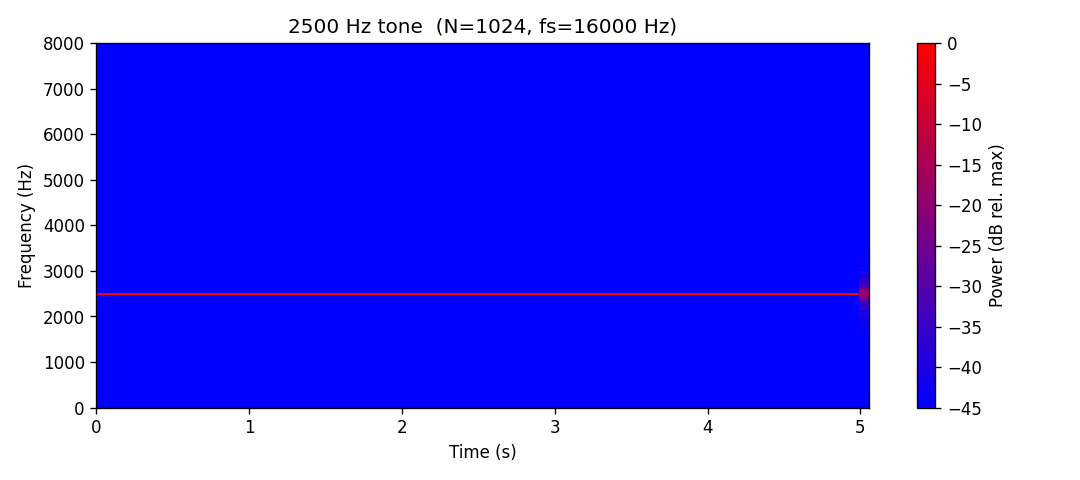
\includegraphics[width=\linewidth]{b_tone2500.png}
  \caption{Spectrograph of the 2500 Hz tone, $F_s = 16$ kHz, $N = 1024$.}
  \label{fig:b}
\end{figure}

The spectrograph shows a single horizontal red line at 2500 Hz that lasts for the whole 5 s. A pure tone has all of its power at one frequency and its amplitude is constant, so the power stays in the same frequency bin in every block. Every other frequency is at the $-45$ dB noise floor (blue). The tone falls exactly on a bin, since $2500 \cdot 1024 / 16000 = 160$, so the power does not leak into neighbouring bins. The small smear at the right end of the plot is the last block, which contains only 128 samples and is padded with zeros, so the abrupt end of the signal spreads its power over nearby frequencies.

\subsection{(c) Spectrograph of the 5000 Hz tone}

Below is the graph that shows the spectrograph of the 5000 Hz tone (Figure~\ref{fig:c}).

\begin{figure}[H]
  \centering
  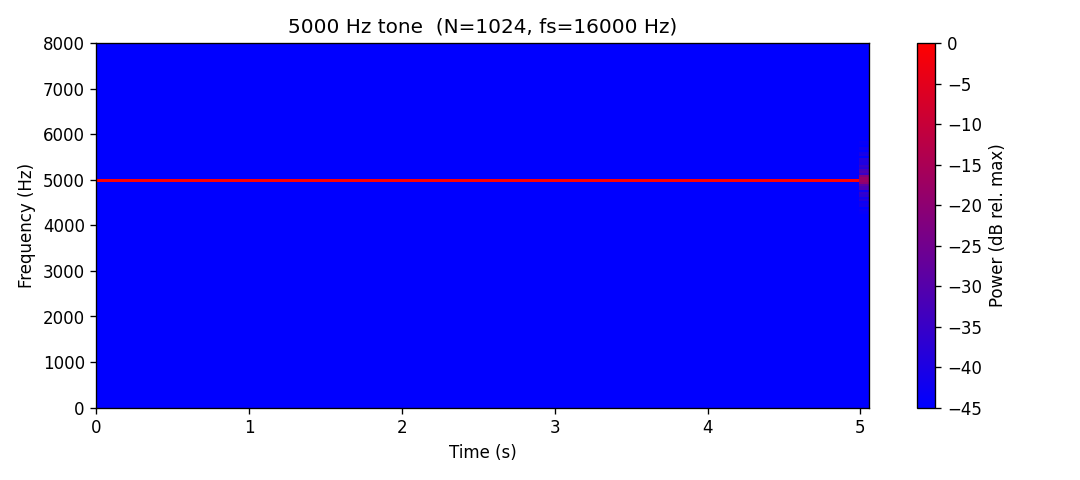
\includegraphics[width=\linewidth]{c_tone5000.png}
  \caption{Spectrograph of the 5000 Hz tone, $F_s = 16$ kHz, $N = 1024$.}
  \label{fig:c}
\end{figure}

The spectrograph shows the same pattern as Figure~\ref{fig:b}, now as a single red line at 5000 Hz (bin $320$) for the whole 5 s, with everything else at the noise floor. Since 5000 Hz is below the Nyquist frequency of 8 kHz, the tone is represented at its true frequency.

\subsection{(d) 5000 Hz tone sub-sampled by 2}

Below is the graph that shows the spectrograph of the 5000 Hz tone after sub-sampling by a factor of 2 without filtering (Figure~\ref{fig:d}). The new sampling rate is 8 kHz.

\begin{figure}[H]
  \centering
  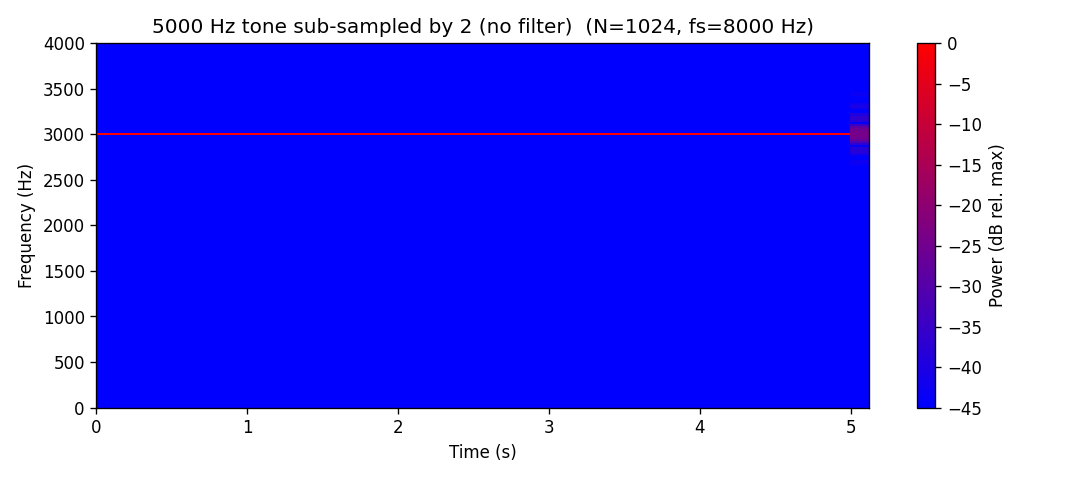
\includegraphics[width=\linewidth]{d_tone5000_sub2.png}
  \caption{Spectrograph of the 5000 Hz tone after sub-sampling by 2 (no filter), $F_s = 8$ kHz, $N = 1024$.}
  \label{fig:d}
\end{figure}

\textbf{Is this what I expect?} Yes. The line is at 3000 Hz and not at 5000 Hz. After sub-sampling, the sampling rate is 8 kHz and the highest representable frequency is 4 kHz, which is why the vertical axis stops at 4 kHz. The 5000 Hz tone is above this limit, so it cannot appear at its own frequency. It aliases to $8000 - 5000 = 3000$ Hz. This follows directly from the samples:
\begin{equation*}
  y[m] = x[2m] = \sin\!\left(2\pi \frac{5000}{16000}\, 2m\right) = \sin\!\left(2\pi \frac{5}{8}\, m\right) = -\sin\!\left(2\pi \frac{3}{8}\, m\right),
\end{equation*}
which is a sine at $\tfrac{3}{8} \cdot 8000 = 3000$ Hz (with inverted sign, which does not change the power).

\textbf{Do the files sound the same?} No. The original file contains a 5 kHz tone and the sub-sampled file contains a 3 kHz tone, so the sub-sampled file is lower in pitch. A tone at 3 kHz was never present in the original signal; it is an artifact of sub-sampling without filtering.

\subsection{(e) Music clip}

The music clip is a 10 s recording at 16 kHz with 16 bits per sample. It is included in the repository as \texttt{Music/music\_play.wav}. Below is the graph that shows its spectrograph (Figure~\ref{fig:e}).

\begin{figure}[H]
  \centering
  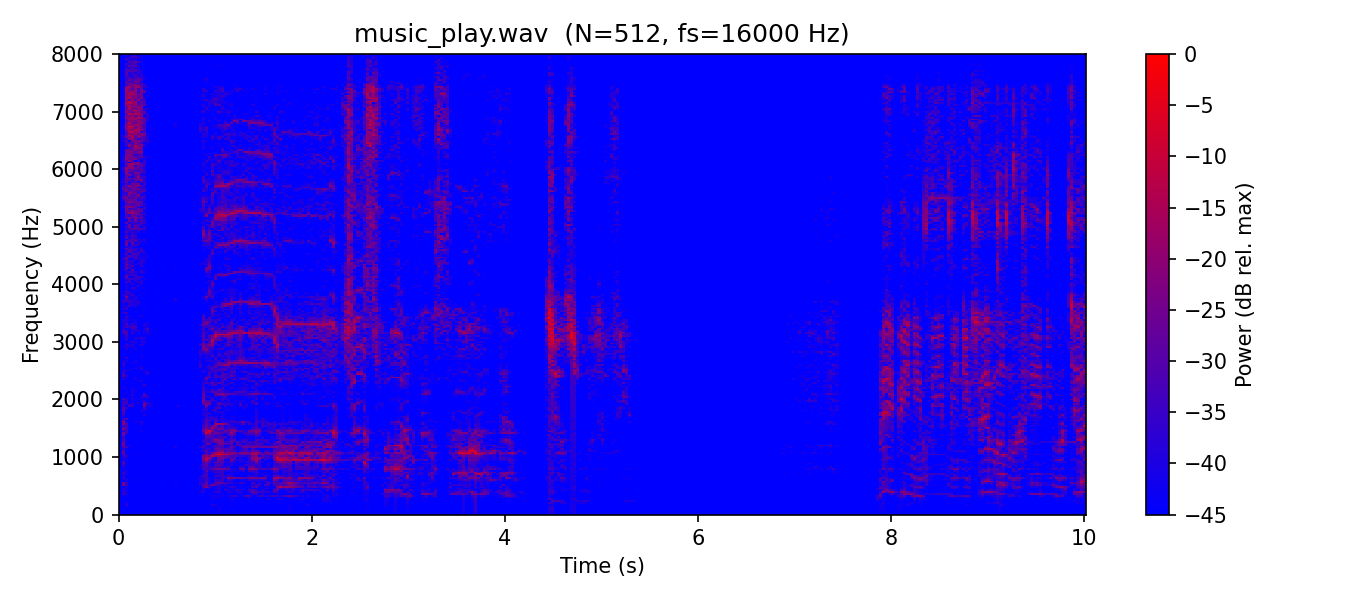
\includegraphics[width=\linewidth]{e_music_spectrograph.png}
  \caption{Spectrograph of the music clip \texttt{music\_play.wav}, $F_s = 16$ kHz, $N = 512$.}
  \label{fig:e}
\end{figure}

\textbf{Can the spectrograph be correlated with the music?} Yes. The features in the display can be matched to the signal in time.
\begin{itemize}
  \item \textbf{Bass and low-frequency notes.} Horizontal lines below about 1.5 kHz, at roughly 500 Hz and 1000 Hz and in between, are sustained low-pitched notes. They are present from about 0.9 s to 4 s and again from about 7.9 s to the end.
  \item \textbf{Treble and harmonics.} Between about 0.9 s and 1.7 s there is a set of evenly spaced horizontal lines that reach up to about 7 kHz. This pattern is consistent with the harmonics of a single sustained note, so the treble content follows the pitch of that note.
  \item \textbf{Sudden events.} Vertical stripes that cover a wide range of frequencies, for example near 2.4 s, 2.6 s, 3.3 s and 4.5 s, are short broadband sounds such as percussive onsets. Their energy is spread over many frequencies and lasts only a few blocks.
  \item \textbf{Quiet section.} Between about 5.4 s and 7.9 s the display is almost entirely blue. The signal level there is very low (the RMS between 6 s and 7 s is about 0.004, compared with about 0.1 in the louder parts), so this passage is nearly silent.
\end{itemize}

\subsection{(f) Sub-sampling the music by 2, 4 and 5 (no filtering)}

Below are the graphs that show the spectrographs of the music after sub-sampling by 2, 4 and 5 without filtering (Figures~\ref{fig:f2}, \ref{fig:f4} and \ref{fig:f5}). In each figure the upper plot is the original and the lower plot is the sub-sampled file. Table~\ref{tab:f} gives the sampling rate of each file, the highest frequency it can represent, and the range of original frequencies that falls above this limit.

\begin{table}[H]
\centering
\begin{tabular}{rrrl}
\toprule
$M$ & New $F_s$ (Hz) & New Nyquist (Hz) & Original content above the limit \\
\midrule
2 & 8000 & 4000 & 4 kHz to 8 kHz \\
4 & 4000 & 2000 & 2 kHz to 8 kHz \\
5 & 3200 & 1600 & 1.6 kHz to 8 kHz \\
\bottomrule
\end{tabular}
\caption{Effect of the sub-sampling factor on the representable frequency range.}
\label{tab:f}
\end{table}

\begin{figure}[H]
  \centering
  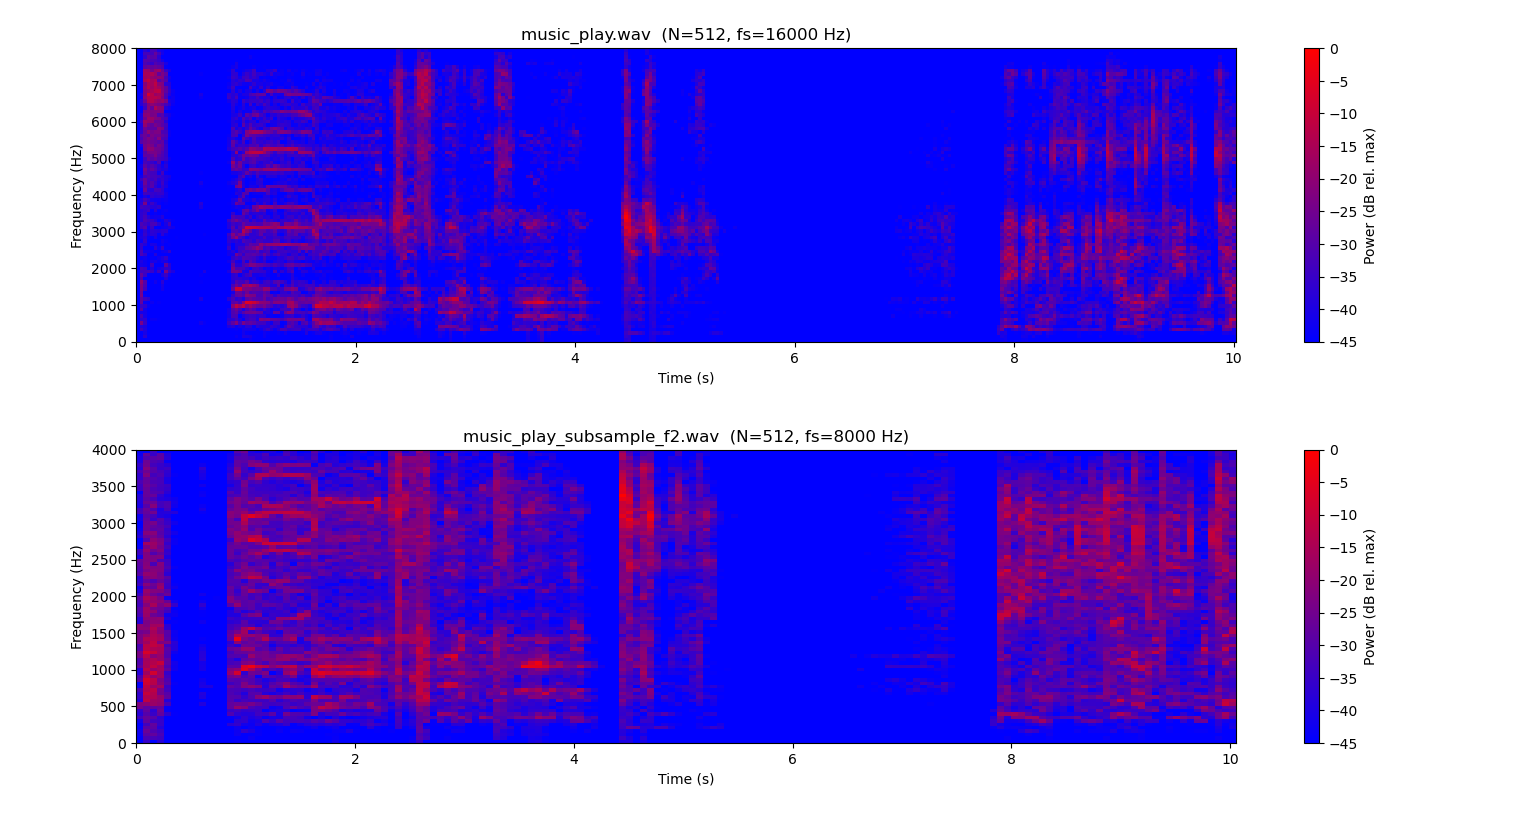
\includegraphics[width=\linewidth]{f_sub2.png}
  \caption{Music sub-sampled by 2 (no filter). Upper: original, $F_s = 16$ kHz. Lower: sub-sampled, $F_s = 8$ kHz.}
  \label{fig:f2}
\end{figure}

\begin{figure}[H]
  \centering
  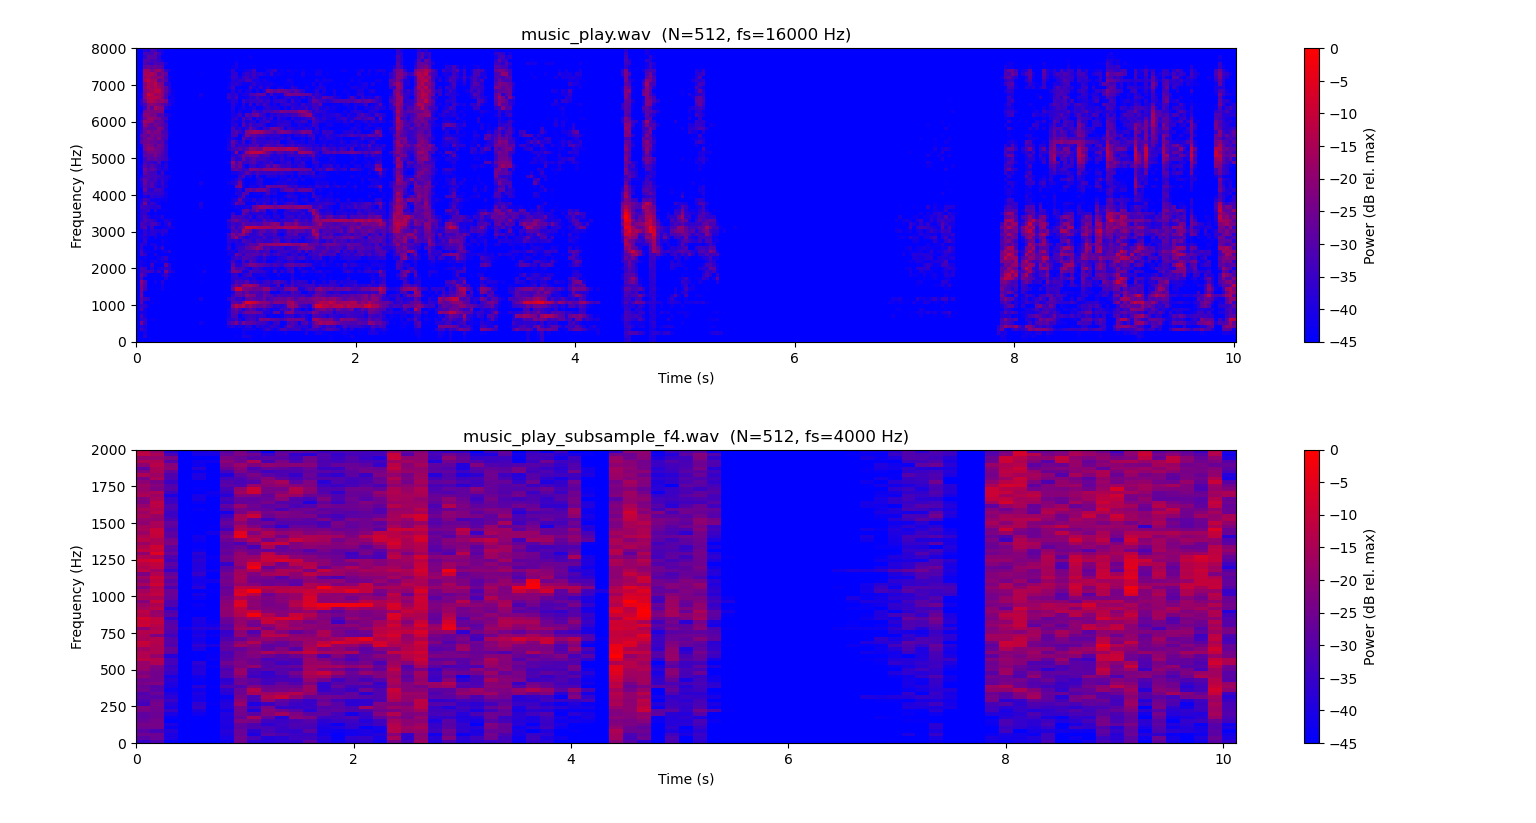
\includegraphics[width=\linewidth]{f_sub4.png}
  \caption{Music sub-sampled by 4 (no filter). Upper: original, $F_s = 16$ kHz. Lower: sub-sampled, $F_s = 4$ kHz.}
  \label{fig:f4}
\end{figure}

\begin{figure}[H]
  \centering
  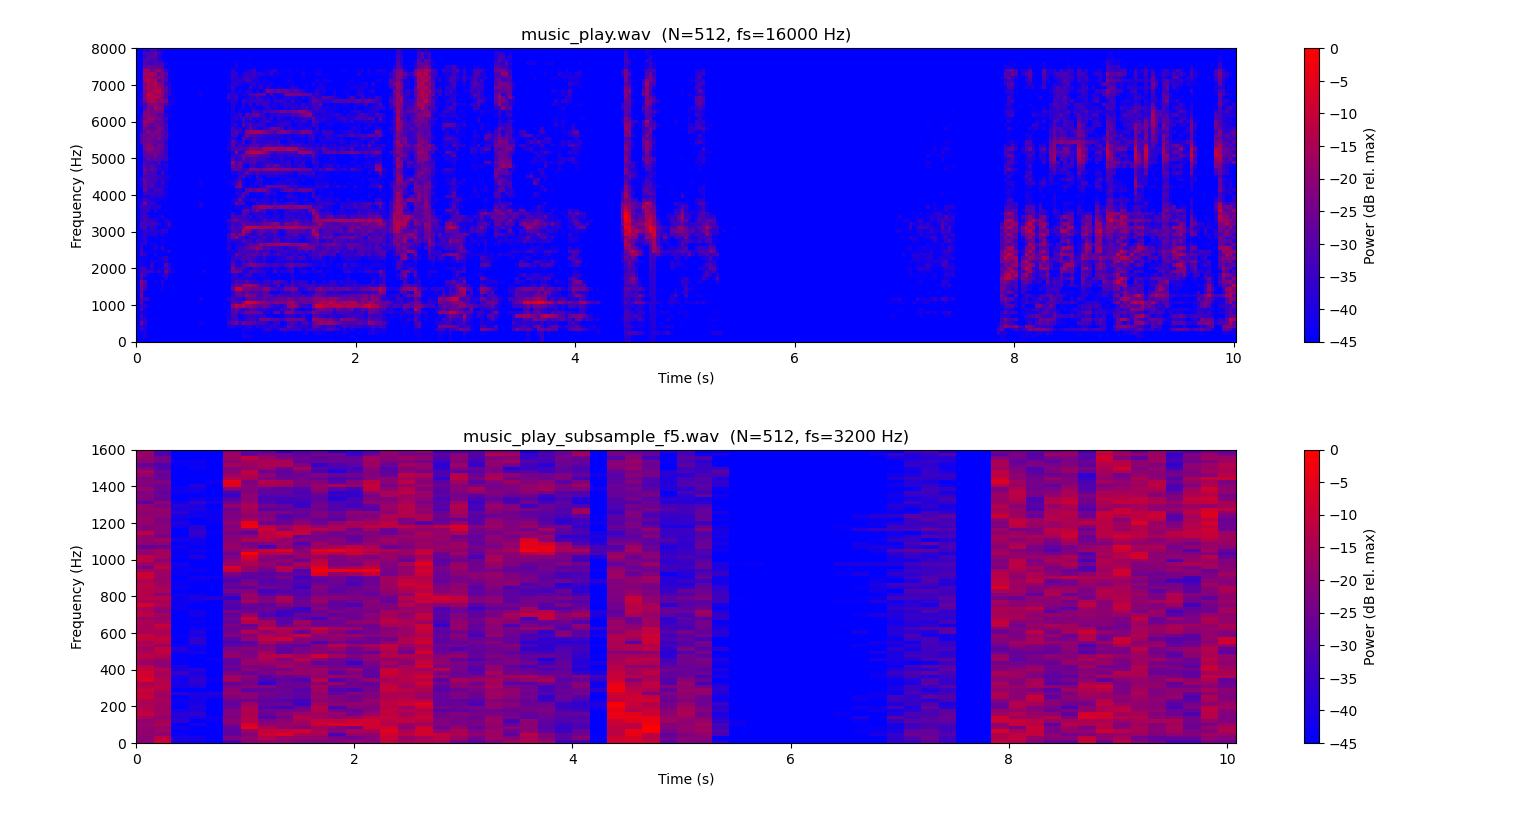
\includegraphics[width=\linewidth]{f_sub5.png}
  \caption{Music sub-sampled by 5 (no filter). Upper: original, $F_s = 16$ kHz. Lower: sub-sampled, $F_s = 3.2$ kHz.}
  \label{fig:f5}
\end{figure}

\textbf{What I hear.} All three sub-sampled files sound clearly degraded and distorted compared with the original. Because each file is written with its own sampling rate, the duration (10.01 s) and the pitch of the music are unchanged. What changes is the content of the sound.

\textbf{What I see.}
\begin{itemize}
  \item \textbf{Factor 2 (Figure~\ref{fig:f2}).} The time structure is unchanged: the loud events and the quiet section are in the same places. The frequency content above 4 kHz in the original does not disappear. It appears in the lower plot between 0 and 4 kHz, mirrored about 4 kHz (a component at frequency $f$ above 4 kHz appears at $8000 - f$). For example, the broadband energy between 5 and 7.5 kHz in the first 0.3 s of the original appears at about 0.5 to 3 kHz in the sub-sampled file. The mirrored harmonic lines are mixed with the real low-frequency lines.
  \item \textbf{Factor 4 (Figure~\ref{fig:f4}).} All content between 2 and 8 kHz, which is three quarters of the original frequency range, is folded into 0 to 2 kHz. The distinct horizontal lines of the original are no longer visible. The whole band is filled with energy, and the display looks like broadband noise.
  \item \textbf{Factor 5 (Figure~\ref{fig:f5}).} The effect is stronger still. The content from 1.6 to 8 kHz is folded into 0 to 1.6 kHz, and almost no tonal structure can be seen. The only parts of the music that remain recognizable are the loud events and the quiet gaps, which are still located at the same times as in the original.
\end{itemize}

\textbf{Observation.} Sub-sampling without a filter preserves when things happen but not which frequencies are present. The larger the factor $M$, the larger the part of the spectrum that is folded, and the more the sub-sampled spectrograph differs from the original. This is aliasing: components above $F_s/(2M)$ are not lost, they reappear at wrong, lower frequencies and add to the genuine content.

\subsection{(g) Low-pass filtering before sub-sampling}

Below are the graphs that show the spectrographs of the music after block-by-block low-pass filtering followed by sub-sampling (Figures~\ref{fig:g2}, \ref{fig:g4} and \ref{fig:g5}). The cutoff is 4 kHz for a factor of 2, 2 kHz for a factor of 4 and 1.6 kHz for a factor of 5. In each figure the upper plot is the filtered file at the original sampling rate of 16 kHz and the lower plot is the filtered file after sub-sampling. In each case the cutoff equals the new Nyquist frequency.

\begin{figure}[H]
  \centering
  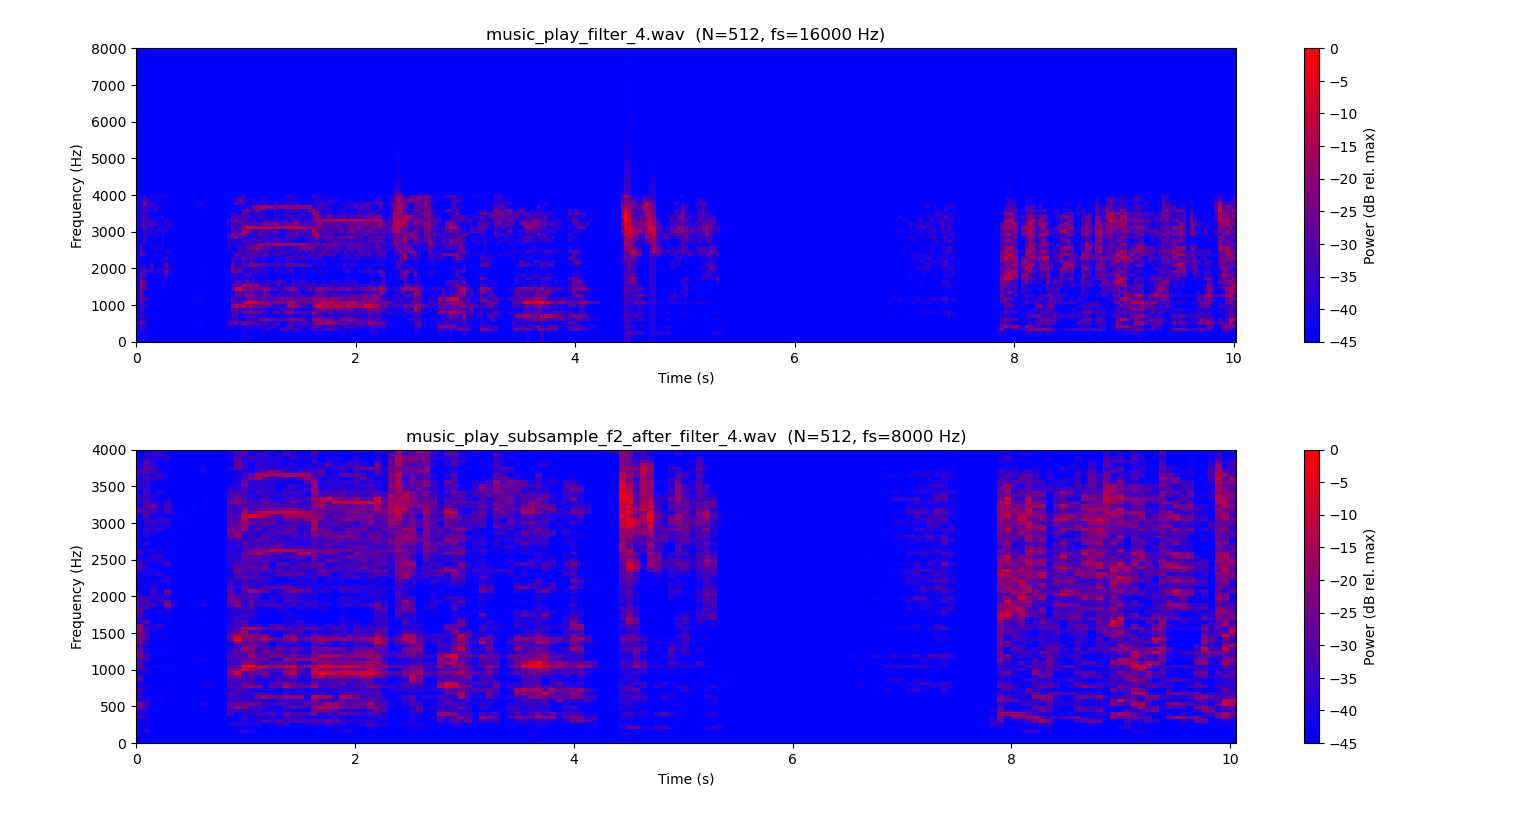
\includegraphics[width=\linewidth]{g_filter4k_sub2.png}
  \caption{Music low-pass filtered at 4 kHz, then sub-sampled by 2. Upper: filtered, $F_s = 16$ kHz. Lower: sub-sampled, $F_s = 8$ kHz.}
  \label{fig:g2}
\end{figure}

\begin{figure}[H]
  \centering
  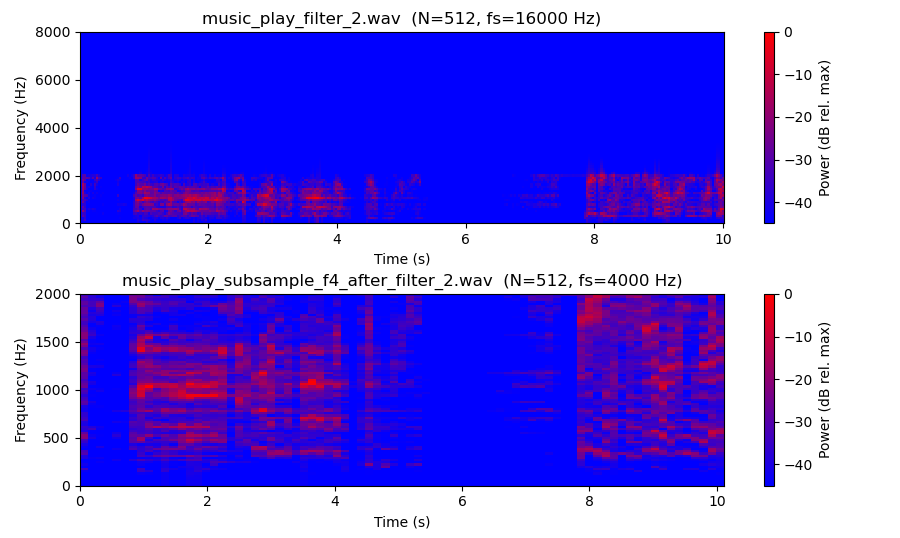
\includegraphics[width=\linewidth]{g_filter2k_sub4.png}
  \caption{Music low-pass filtered at 2 kHz, then sub-sampled by 4. Upper: filtered, $F_s = 16$ kHz. Lower: sub-sampled, $F_s = 4$ kHz.}
  \label{fig:g4}
\end{figure}

\begin{figure}[H]
  \centering
  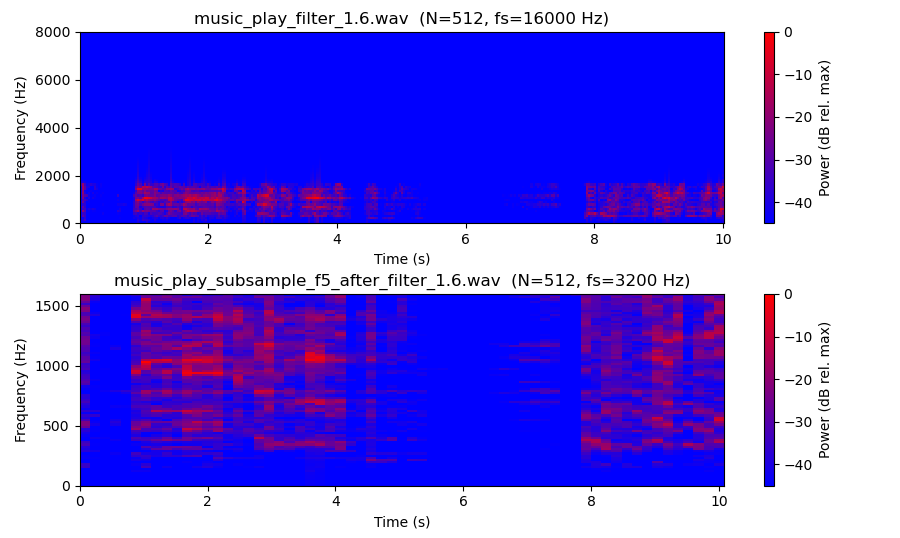
\includegraphics[width=\linewidth]{g_filter1_6k_sub5.png}
  \caption{Music low-pass filtered at 1.6 kHz, then sub-sampled by 5. Upper: filtered, $F_s = 16$ kHz. Lower: sub-sampled, $F_s = 3.2$ kHz.}
  \label{fig:g5}
\end{figure}

\textbf{What I see.} In the upper plot of each figure there is no energy above the cutoff frequency, and the content below the cutoff is the same as in the original (Figure~\ref{fig:e}). In the lower plots the sub-sampled spectrographs keep the distinct horizontal lines of the original low-frequency notes, for example the lines near 1 kHz and the harmonics near 3 kHz in Figure~\ref{fig:g2}. Nothing is mirrored or folded into the band, and the quiet section is still empty. This contrasts with Figures~\ref{fig:f2}, \ref{fig:f4} and \ref{fig:f5}, where the same sub-sampling without filtering produced extra content and, for factors 4 and 5, hid the tonal structure completely.

\textbf{Do they sound the same as the part (f) files?} No. The filtered files sound cleaner. They are duller than the original because everything above the cutoff has been removed, but they do not contain the distortion that is heard in the part (f) files.

\textbf{Which do I prefer?} I prefer the files that were filtered before sub-sampling. They are a reduced version of the original: only content that the lower sampling rate can represent remains, and it is at its true frequency. Without filtering, content above the new Nyquist frequency is folded onto the music and cannot be separated from it afterwards. Removing it first, as the low-pass filter does, is the only way to avoid this once the sampling rate is reduced.

% -------------------------------------------------------
% REPOSITORY CONTENTS
% -------------------------------------------------------
\section{Repository Contents}

The GitHub repository \href{\repourl}{\texttt{\repourl}} contains the following.
\begin{itemize}
  \item The application source code (\texttt{main.py}, \texttt{dsp/}, \texttt{audio/}, \texttt{ui/}) and its tests.
  \item The tone files for part (a) in \texttt{out/tones}.
  \item The music clip and all sub-sampled and filtered audio files for parts (e), (f) and (g) in \texttt{Music/}.
  \item The requirements documents, the design document and the interrogation file.
  \item The source of this report in \texttt{latex/}.
\end{itemize}

\end{document}
